% This is "sig-alternate.tex" V1.9 April 2009
% This file should be compiled with V2.4 of "sig-alternate.cls" April 2009
%
% This example file demonstrates the use of the 'sig-alternate.cls'
% V2.4 LaTeX2e document class file. It is for those submitting
% articles to ACM Conference Proceedings WHO DO NOT WISH TO
% STRICTLY ADHERE TO THE SIGS (PUBS-BOARD-ENDORSED) STYLE.
% The 'sig-alternate.cls' file will produce a similar-looking,
% albeit, 'tighter' paper resulting in, invariably, fewer pages.
%
% ----------------------------------------------------------------------------------------------------------------
% This .tex file (and associated .cls V2.4) produces:
%       1) The Permission Statement
%       2) The Conference (location) Info information
%       3) The Copyright Line with ACM data
%       4) NO page numbers
%
% as against the acm_proc_article-sp.cls file which
% DOES NOT produce 1) thru' 3) above.
%
% Using 'sig-alternate.cls' you have control, however, from within
% the source .tex file, over both the CopyrightYear
% (defaulted to 200X) and the ACM Copyright Data
% (defaulted to X-XXXXX-XX-X/XX/XX).
% e.g.
% \CopyrightYear{2007} will cause 2007 to appear in the copyright line.
% \crdata{0-12345-67-8/90/12} will cause 0-12345-67-8/90/12 to appear in the copyright line.
%
% ---------------------------------------------------------------------------------------------------------------
% This .tex source is an example which *does* use
% the .bib file (from which the .bbl file % is produced).
% REMEMBER HOWEVER: After having produced the .bbl file,
% and prior to final submission, you *NEED* to 'insert'
% your .bbl file into your source .tex file so as to provide
% ONE 'self-contained' source file.
%
% ================= IF YOU HAVE QUESTIONS =======================
% Questions regarding the SIGS styles, SIGS policies and
% procedures, Conferences etc. should be sent to
% Adrienne Griscti (griscti@acm.org)
%
% Technical questions _only_ to
% Gerald Murray (murray@hq.acm.org)
% ===============================================================
%
% For tracking purposes - this is V1.9 - April 2009

\documentclass{sig-alternate}
  \pdfpagewidth=8.5truein
  \pdfpageheight=11truein

\makeatletter
\newif\if@restonecol
\makeatother
\let\algorithm\relax
\let\endalgorithm\relax


\usepackage{multirow}	% for tables
\usepackage{graphicx}   % for including EPS
\usepackage{rotating}
\usepackage{url}

% % % Special mathematical fonts
\usepackage{amssymb}
\usepackage{amsmath}
\usepackage{amsfonts}
\usepackage{bm}
\usepackage{srctex}
\usepackage[linesnumbered,algo2e,noend]{algorithm2e}
\usepackage{algpseudocode}
\usepackage{setspace}
%\usepackage[compact]{titlesec}
%\usepackage{mdwlist}
%\usepackage[left=2cm,top=1cm,right=2cm,nohead,nofoot]{geometry}

\algnotext{EndFor}
\algnotext{EndIf}

\begin{document}
%
% --- Author Metadata here ---
\conferenceinfo{SAC'13}{March 18-22, 2013, Coimbra, Portugal.}
\CopyrightYear{2013} % Allows default copyright year (2002) to be over-ridden - IF NEED BE.
\crdata{978-1-4503-1656-9/13/03}  % Allows default copyright data (X-XXXXX-XX-X/XX/XX) to be over-ridden.
% --- End of Author Metadata ---

\title{Out-Of-Bag Discriminative Graph Mining}
%
% You need the command \numberofauthors to handle the 'placement
% and alignment' of the authors beneath the title.
%
% For aesthetic reasons, we recommend 'three authors at a time'
% i.e. three 'name/affiliation blocks' be placed beneath the title.
%
% NOTE: You are NOT restricted in how many 'rows' of
% "name/affiliations" may appear. We just ask that you restrict
% the number of 'columns' to three.
%
% Because of the available 'opening page real-estate'
% we ask you to refrain from putting more than six authors
% (two rows with three columns) beneath the article title.
% More than six makes the first-page appear very cluttered indeed.
%
% Use the \alignauthor commands to handle the names
% and affiliations for an 'aesthetic maximum' of six authors.
% Add names, affiliations, addresses for
% the seventh etc. author(s) as the argument for the
% \additionalauthors command.
% These 'additional authors' will be output/set for you
% without further effort on your part as the last section in
% the body of your article BEFORE References or any Appendices.

\numberofauthors{3} %  in this sample file, there are a *total*
% of EIGHT authors. SIX appear on the 'first-page' (for formatting
% reasons) and the remaining two appear in the \additionalauthors section.
%
\author{
% You can go ahead and credit any number of authors here,
% e.g. one 'row of three' or two rows (consisting of one row of three
% and a second row of one, two or three).
%
% The command \alignauthor (no curly braces needed) should
% precede each author name, affiliation/snail-mail address and
% e-mail address. Additionally, tag each line of
% affiliation/address with \affaddr, and tag the
% e-mail address with \email.
%
% 1st. author
\alignauthor
Andreas Maunz\\
       \affaddr{Institute for Physics}\\
       \affaddr{Hermann-Herder-Str. 3}\\
       \affaddr{79194 Freiburg, Germany}\\
       \email{andreas@maunz.de}
% 2nd. author
\alignauthor David Vorgrimmler\\
       \affaddr{in-silico Toxicology}\\
       \affaddr{Altkircherstr. 4}\\
       \affaddr{4054 Basel, Switzerland}\\
       \email{vorgrimmler@in-silico.ch}
% 3rd. author
\alignauthor 
Christoph Helma\\
       \affaddr{in-silico Toxicology}\\
       \affaddr{Altkircherstr. 4}\\
       \affaddr{4054 Basel, Switzerland}\\
       \email{helma@in-silico.ch}
}

\maketitle
\begin{abstract}
  In class-labeled graph databases, each graph is associated with one from a
finite set of classes, which induces associations between the classes and subgraphs
occurring in the database graphs. The subgraphs with strong
class associations are called discriminative subgraphs. In this work,
discriminative subgraphs are repeatedly mined on bootstrap samples of a graph
database in order to estimate subgraph associations more precisely than 
without sampling. The number of times a subgraph occurs in a graph associated with each class
(support values)
are recorded over the out-of-bag instances of the bootstrap process. We investigate two different
methods for the approximation of the true underlying support values from these
empirical values, involving sample mean and maximum likelihood estimation. We
show that both significantly improve on the process, compared to single
runs of discriminative graph mining, by applying the methods to
publicly available toxicological datasets, and validating support values, class bias, and 
class significance. In toxicology,
the detection of subgraphs (fragments of chemical structure) that induce toxicity is a major goal.
Apart from the subgraph associations being
statistically validated, the number of subgraphs created by the proposed methods are
much lower than for ordinary discriminative graph mining, which is often a bottleneck in the
application of computation models to such datasets, and hinders interpretation of the results.
\end{abstract}



% A category with the (minimum) three required fields
\category{H.2.8}{Database Applications}{Data Mining, Statistical Databases}
\terms{Theory, Experimentation, Performance}

\section{Introduction}
\label{s:Introduction}
Given a class-labeled graph database, discriminative graph mining is a
supervised learning task with the goal to extract graph fragments (subgraphs)
with strong associations to the classes, according to statistical constraints
set by the user. For example, the subgraphs may be molecular fragments that
induce toxicity. Indeed, finding such fragments is a major goal in toxicology
\cite{kazius05derivation}. However, discriminative graph mining yields large
result sets, even for very high thresholds on subgraph class associations \cite{Jun04Spin}. 
Moreover, it is an unstable
process, i.e. slight changes in the sample may lead to substantially different subgraph
sets. 

%A bagged predictor consists of several aggregate predictors, each trained on a
%dedicated bootstrap sample of the training data. Bagged predictors have the
%potential for considerably higher predictive accuracy, compared to single
%predictors, especially in the context of unstable prediction methods
%\cite{breiman96oob}. For example, out-of-bag estimation of node errors in
%decision trees could improve on estimates obtained from the training data as a
%whole \cite{breiman96oob}. Bagged predictor estimates may be obtained from the out-of-bag
%instances, which saves computational effort compared to crossvalidation on the
%bootstrap samples. 

In statistical learning, a bagged predictor consists of several aggregate
predictors, each trained on a dedicated bootstrap sample of the training
instances. As bootstrapping draws instances with replacement, $1/e$ (roughly 37
\%) of instances are not drawn in each sample, on average. These instances
(referred to as out-of-bag instances) may be used to obtain estimates of the
bagged predictor, by letting each predictor in the bag vote on ``his'' corresponding 
out-of-bag instances, 
which are test examples unknown to the predictor.
For example, out-of-bag estimation of node errors in
decision trees could improve on estimates obtained from the training data as a
whole \cite{breiman96oob}.

This work extends discriminative subgraph mining by out-of-bag estimation of 
subgraph occurrence frequencies in the graphs associated with each class (support values), 
and by aggregating subgraphs in the output that pass the
statistical constraints. Infrequently occurring subgraphs are filtered out, 
which removes the instability to a large extent. 
This yields statistically validated, highly significant,
discriminative subgraphs, which may be useful for diagnostic or predictive
modelling, or for expert inspection. 

The remainder of this work is structured as follows: We present related work
with a focus on discriminative graph mining (section \ref{s:relatedWork}), our
proposed methods for out-of-bag estimation of support values, as
well as algorithmic implementation (section \ref{s:Methods}).
Experiments include validation of subgraph support
values, $p$-values, and class bias on publicly available databases of
various sizes and numbers of classes (section \ref{s:Experiments}).
We draw conclusions in section \ref{s:Conclusion}.
The contributions are summarized as follows:
\begin{itemize}
  \item Repeated discriminative graph mining on bootstrap samples of a
    class-labeled graph database is proposed as a means to stabilize estimates
    for subgraph properties, such as support values per class, compared to
    single runs of discriminative graph mining. The estimation is performed
    using the out-of-bag instances of the individual bootstrap samples.
  \item Two methods for the estimation of support values are described, where both
    handle multiple class values. Significance tests are applied to these
    estimated values and insignificant subgraphs are removed from the results. 
  \item The estimated support values, class significance values, and class
    biases are empirically validated on molecular databases of various
    sizes. The results indicate significant improvements over 
    ordinary discriminative graph mining, where the effect is generally larger the
    smaller the datasets are. We conclude that out-of-bag estimation has 
    potential to generate concise, discriminative subgraph sets for
    use in statistical models and/or expert inspection.
\end{itemize}


\section{Related Work}
\label{s:relatedWork}

Out-of-bag methods have been used to robustly estimate node probabilities and
node error rates in decision trees \cite{breiman96oob} as well as the
generalization error and accuracy of bagged predictors. In the work by Bylander
\cite{bylander02estimating}, generalization error was well modeled by
out-of-bag estimation, and its already small bias could be further reduced by a
correction method, where, in order to correct the prediction of a given
instance, similar out-of-bag instances with the same class were
employed. However, the method of out-of-bag estimation is not confined to these
examples, and may be used to estimate other statistical properties in
supervised learning.

Discriminative graph mining is often employed as a preprocessing step to
statistical learning, because discriminative subgraphs may be useful as descriptors
\cite{bringmann10lego}. Nowadays, there is a variety of well-known statistical
learning algorithms available ``off the shelf'', which makes a workflow
attractive where subgraphs are extracted from the data, represented in a
unified format, and fed into a machine learning algorithm \cite{KRH01}.
Usually, discriminative subgraphs are mined from a graph database using a
predefined threshold with regard to target class associations. A subgraph
qualifies for the result set if it passes a corresponding significance test.
However, such approaches tend to produce huge sets of very similar subgraphs,
even with very high thresholds on discriminative potential, which would prevent
machine learning methods from building models in acceptable time, and post-processing 
would be required to lower redundancy and eliminate the vast
majority of subgraphs \cite{Hasan_origami:mining,Jun04Spin}. Moreover, the
result is not stable with regards to perturbations of the database.

Subgraph boosting \cite{saigo09gboost} is an integrated approach to build models on
small sets of subgraphs, alternating between graph mining and model building. The method presented here is clearly
different from boosting, because it calculates subgraphs independently from a specific model. It is similar in that it calculates a small
collection of discriminative subgraphs, but it is also stable against
perturbations of the database, which is generally not the case for boosting.


\section{Methods}
\label{s:Methods}

\subsection{Basic Graph Theory}
\label{ss:BasicGraphTheory}
A graph database is a tuple $(G, \Sigma, a)$, where $G$ is a set of graphs,
$\Sigma \ne \emptyset$  is a totally ordered set of labels and $a: G
\rightarrow I$, $I \subset \mathbb{N}$, is a surjective function that assigns one from a
finite set of class values to every graph in the database. The set 
$I$ consists of at least two values, and for all $i \in I$, the set that contains all $g \in G$
with $a(g)=i$ is called $G^i$. We consider labeled, undirected
graphs, i.e. tuples $g=(V,E,\Sigma,\lambda)$, where $V\ne \emptyset$ is a
finite set of nodes and $E \subseteq V = \{\{v_1, v_2\} \in \{V \times V\}, v_1
\ne v_2\}$ is a set of edges and $\lambda: V\cup E \rightarrow \Sigma$ is a
label function. 
An ordered set of nodes $\{ v_1, \ldots, v_m\}$ is a \emph{path} between $v_1$ and $v_m$, if $\{v_i, v_{i+1}\} \in E, i \in \{1,\ldots,m-1\}$ and $v_i \neq v_j$ for all $i,j\in \{1,\ldots,m\}$.
We only consider connected graphs here, i.e. there is a path
between each two nodes in the graph.

A graph $g'=(V',E',\Sigma',\lambda')$ subgraph-isomorphic to $g$ if $V'
\subseteq V$ and $E' \subseteq E$ with $V' \ne \emptyset$ and $E' \ne
\emptyset$, $\lambda'(v_1)=\lambda(v_2)$ whenever $v_1=v_2$, and
$\lambda'(e_1)=\lambda(e_2)$ whenever $e_1=e_2$, for all nodes and edges in
$g'$. In this case, graph $g'$ is also referred to as a subgraph of $g$ -- we also say
that $g'$ covers $g$. The subset of the database instances $G$ that $g'$
covers is referred to as the occurrences of $g'$, and its size as (total) support of
$g'$, denoted $support(g')$. As a special case, the size of the subset of occurrences with $a(g)=i$,
for any $g$ in the occurrences, is referred to as the support of $g'$ for class
$i$. Thus, any subgraph has associated support values per class, ranging each
between 0 and the support of $g'$, and summing up to the support of $g'$.

The subgraphs considered in this work are free subtrees. Here, we define a tree
as a graph with exactly $n-1$ edges that connect its $n$ nodes. A free tree is
a tree without a designated root node. For an introduction to tree mining and
the terminology used there, see the overview by Chi \emph{et al.}
\cite{CMNK01Frequent}.

\subsection{Significance Test}
\label{ss:significance-test}
% general chisq test
For a given subgraph $g$, we seek a $|I| \times 2$ contingency table that lists the
support values per class in the first column and the overall distribution of target
classes in the second column, as in Table \ref{t-ContingencyTableIndTest}.
\begin{table}[t]
  \centering
  \begin{tabular}{|l|l|l|}
    \hline
    ~           &	$g$       & $all$       \\\hline
    class 1	    &	$k_1$     & $|G^1|$     \\\hline
    class 2 	  &	$k_2$     & $|G^2|$     \\\hline
    $\ldots$ 	  &	$\ldots$  & $\ldots$    \\\hline
    class $|I|$	&	$k_{|I|}$ & $|G^{|I|}|$ \\\hline
    $\Sigma$	  &	$k$       & $|G|$       \\\hline
  \end{tabular}
  \caption[]{Contingency table for subgraph $g$.}
  \label{t-ContingencyTableIndTest}
\end{table}
This data serves to check whether $g$'s support values differ
significantly from the overall class distribution. The $\chi^2_d$ function for
distribution testing, defined as
\begin{equation}
  %\chi^2_d(x,y) = \frac{(y-\frac{xm}{n})^2}{\frac{xm}{n}} + \frac{(x-y-\frac{x(n-m)}{n})^2}{\frac{x(n-m)}{n}},
  \chi^2_d(x,y) = \sum_{i=1}^{|I|} \frac{(k_i-E(k_i))^2}{E(k_i)},
  \label{eq:chid}
\end{equation} 
where $E(k_i)=\frac{|G^{i}| k}{|G|}$ is the expected value of $k_i$, calculates
the sum of squares of deviations from the expected support for all target
classes. The function value is then compared against the $\chi^2$
distribution function and conduct a significance test with
$|I|-1$ degrees of freedom to obtain a $p$-value $p(g)$. 
%The $|G^{i}|$ entries are constants and take the values of
%the overall $|G^{i}|$. 
%This is possible due to the stratified bootstrapping approach,
%which maintains the overall class proportions in each sample (see section
%\ref{ss:oob-dgm}). 
Additionally, the bias of $g$ is determined as $\arg\max_i (\frac{k_i}{k}/\frac{G^i}{G})$, to designate the dominant class for $g$.
%The next sections discuss methods to obtain the
%$k_i$ entries in the table from the support values obtained during bootstrapping (section
%\ref{ss:oob-dgm}). 

\subsection{Out-Of-Bag Discriminative Graph Mining}
\label{ss:oob-dgm}
In ordinary discriminative graph mining, the task is to find all subgraphs
$g$ with $support(g)>minsup$ and $p(g)<\alpha$, where $minsup$ and $\alpha$ are
set by the user.
%Our proposed method splits $G$
%into stratified, equal-sized training and test databases $G_{Train}$ and $G_{Test}$.
Out-of-bag discriminative graph mining is different, in that bootstrapping is repeatedly performed on $G$.
In each bootstrap sample $G'$, it is ensured that $\vert G^i\vert$ graphs are associated with
class $i$, by drawing with replacement and uniform probability inside 
class $i$, for all $i$ in $I$ (stratification). 
%On average, about 37\% (1/$e$) of training instances 
%will not be drawn in any bootstrap sample (out-of-bag instances). 
Ordinary discriminative graph mining is applied to the database induced by $G'$, with $minsup$ and $\alpha$ thresholds. 
%Each subgraph in the result set has associated support values, $p$-value, 
%and bias, as calculated on the bootstrap sample.
Finally, subgraph support values are assessed by performing isomorphism
tests on the out-of-bag instances (``matching'').

More specifically, bootstrapping and graph mining is repeated $N$ times, where in each
iteration, pairs of subgraphs and out-of-bag support values per class
$(g,k_1,\ldots,k_{\vert I\vert})$ are produced, meaning that subgraph $g$
occurs in $k_i$ out-of-bag graphs associated with class $i$. The results are
recorded over the $N$ bootstrap samples, such that for each $g$, the list of
support values is a tuple $(\mathbf{k_1}\ldots\mathbf{k_{\vert I\vert}})$,
where $\mathbf{k_i}$ is a vector $(k_i^1\ldots k_i^N)$, containing all the
support values. 
The vectors $\mathbf{k_i}$
are generally sparse (contain missing values), due to the instability of discriminative graph mining,
i.e. perturbations to the dataset (such as bootstrap sampling) yield almost
always a different (but partially overlapping) selection of subgraphs. 
The missing values occupy the same indices in the $\mathbf{k_i}$.
To cope with the
variety of rare subgraphs, a fixed threshold removes all subgraphs with less
than $\lfloor0.3*N\rfloor$ entries in the list of support values, after the end
of bootstrapping.
For the remaining ones, the total support is determined from the class specific support values by
summing up vectors $\mathbf{k_i}$ across classes (ignoring indices with missing entries):
$\mathbf{k}=\sum_{i=1}^{\vert I\vert} \mathbf{k_i}$. 

From the recorded results, support values are estimated. Two methods are described in the next sections, based either
on the sample mean support per class, and using data of the current subgraph
only, or on a maximum likelihood estimate, involving some of the other
subgraphs. Then the significance test from section \ref{ss:significance-test}
is run on the estimated support values, yielding estimated class significance values ($p$-values), 
and biases.

\subsubsection{Sample Mean Method}
\label{ss:simple-mean}
We set the value of $k_i$ in Table \ref{t-ContingencyTableIndTest} to
$\overline{\mathbf{k_i}}$, i.e. the sample mean
across the entries of vector $\mathbf{k_i}$ (ignoring missing values), for all $i \in \{1,\ldots,|I|\}$,
and $k$ is the sum of the $k_i$.

\subsubsection{Maximum Likelihood Estimation Method}
\label{ss:MLE}
Here, we employ some of the other subgraphs to form estimates for the $k_i$.
The first step in this process is to extract the subgraphs with the same class
bias as $g$ (see section \ref{ss:significance-test}). Local ties are broken in
favor of the dominant global class. In case of a further tie on the global
level, one of the globally dominant classes is chosen with uniform probability.
In a second step, the subgraphs with the same class bias as $g$ are used to correct
$g$'s local frequencies by weighting. This approach has some similarity to the
work by Bylander \cite{bylander02estimating}, however, his aim is to correct
instance predictions, and his correction employs similar out-of-bag instances,
whereas our correction happens across bootstraps, and on the subgraphs (not
instances) obtained collectively from all the bootstrap samples. For each
class, we model the event that each $k_i^j \in \mathbf{k_i}$ would occur for
each of the subgraphs with the same class bias as $g$ as a multinomial
selection process. More specifically, we determine the class probabilities for
each subgraph $g'$ with the same class bias as $g$ with a maximum likelihood
estimator. It is the smoothed vector of relative class specific support values,
defined as:
\begin{equation}
  \mathbf{\alpha_{g'}} = \left(\frac{1+\vert\mathbf{k_1}\vert_1}{\vert I\vert+\vert\mathbf{k}\vert}_1,\ldots,\frac{1+\vert\mathbf{k_{\vert I\vert}}\vert_1}{\vert I\vert+\vert\mathbf{k}\vert_1}\right)
  \label{eqn:mlexpr}
\end{equation}
where the $\mathbf{k_i}$ and $\mathbf{k}$ pertain to $g'$, and $\vert\cdot\vert_1$ is the one-norm (the sum of the vector elements, ignoring missing values). Following that, for
each non-missing tuple $(k_1^j,\ldots,k_{\vert I\vert}^j)$ pertaining to $g$, a probability distribution is
determined from this collection of multinomials:
\begin{equation}
  p((k_1^j,\ldots,k_{\vert I\vert}^j))=\frac{\sum_{g'} p((k_1^j,\ldots,k_{\vert I\vert}^j); \mathbf{\alpha_{g'}})}{\sum_{g'}1}
  \label{eqn:avgpr}
\end{equation}
Finally, the $k_i^j$ values pertaining to $g$ are corrected in a weighted average
based on this probability distribution:
\begin{equation}
  \overline{\mathbf{k_i}}=\frac{\sum_j k_i^j p((k_1^j,\ldots,k_{\vert I\vert}^j))}{\sum_j p((k_1^j,\ldots,k_{\vert I\vert}^j))}
  \label{eqn:avgki}
\end{equation}
Again, we set the value of $k_i$ in Table \ref{t-ContingencyTableIndTest} to $\overline{\mathbf{k_i}}$.

\subsection{Algorithm}
\label{s:Algorithm}
%\begin{figure*}[t]
%  \begin{center}
%    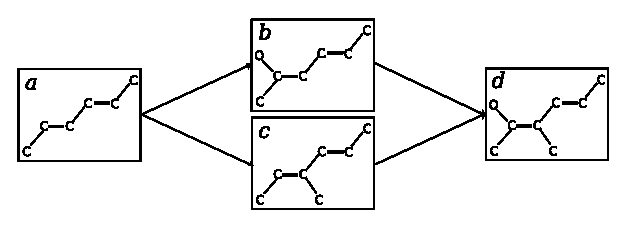
\includegraphics[width=9cm]{classes.eps}
%  \end{center}
%  \caption{Two non-disjoint partitions $(a,b,d)$ and $(a,c,d)$. The members are ordered by subgraph relationship.}
%  \label{fig:bbrc}
%\end{figure*}
%According to section \ref{ss:oob-dgm}, graph mining proceeds in two steps:
%mining the given bootstrap sample and -- for each subgraph found -- looking up
%support values per class by matching on the out-of-bag instances. 
Ordinary discriminative graph mining may be 
implemented using a discriminative graph mining algorithm of choice as ``mother algorithm''. Here, we
employ backbone refinement class mining (BBRC) \cite{maunz11efficient}. It
achieves a certain degree of compression by partitioning the subgraph search space into non-disjoint sets (classes) with the same
longest paths (backbones) and selecting only one representative from each
class. 
%Inside each partition, the patterns are ordered by the subgraph relationship (see figure \ref{fig:bbrc}). 
The representative is chosen to minimize the $p$-value (section \ref{ss:significance-test}), unless no member passes the user-defined significance constraint, in which case no representative is chosen.
In any case, the search is bounded by minimum total support and significance threshold $\alpha$.
%The search is also bounded by minimum total support, as described in section \ref{ss:oob-dgm}.
In the BBRC output, two isomorphic subgraphs are always represented by the same string identifier.
The strings are SMARTS, a kind of regular expression to encode
molecular fragments as strings\footnote{see \url{http://www.daylight.com/dayhtml/doc/theory/theory.smarts.html}}. This approach allows to store out-of-bag support values $\mathbf{k_i}$ in a
hash structure, using SMARTS as keys. 

\begin{algorithm2e*}[t]
  \fontsize{8}{10}
  \selectfont
  \KwData{$dataBase, numBoots, minHashLength, method, minSup$}
  \KwResult{$[subgraphs, values]$ \text{; $values$ include support, $p$-value, and bias}}
  \If{$method=$\text{ODGM}}{
     $[subgraphs, values] \leftarrow BBRC(dataBase, minSup, 0.05)$\;
  }
  \Else{
    $hashTable \leftarrow \{\}$\;
    \For{$i:=1 \to numBoots$ (Parallel Processing)} { 
      $sample,OOB \leftarrow drawBsSample(dataBase)$\;
      $[subgraphs, values] \leftarrow BBRC(sample, minSup, 0.05)$\;
      $insert(hashTable,match(subgraphs,OOB))$\;
    }
    $[subgraphs, values] \leftarrow []$\;
    \For{$subgraph \in keys(hashTable)$}{
      \If{$length(hashTable[subgraph]) \geq minHashLength$}{
         $[candidateSupportValues, candidatePValue, candidateBias] \leftarrow method(hashTable[subgraph])$\;
        \If{$candidatePValue < 0.05$}{
          $subgraphs \leftarrow subgraphs \cup subgraph$\;
          $values \leftarrow values \cup [candidateSupportValues, candidatePValue, candidateBias]$\;
        }
      }
    }
  }
  \caption{Calculation of subgraph significance on out-of-bag instances\label{alg:bbrc-sample}}
\end{algorithm2e*}
Algorithm \ref{alg:bbrc-sample} switches between out-of-bag estimation and ordinary discriminative graph mining (ODGM), where 
the significance parameter $\alpha$ was kept fixed at 0.05 at all times.
We describe out-of-bag estimation first. Line 4
creates a hash table to gather results from mining bootstrap samples 
(line 7). The resulting subgraphs are matched on the out-of-bag instances (line
8), and the results are stored in the hash. On termination of the loop, each hash
entry $\mathbf{k_i}$ has at most $N$ support values. Post-processing the results
incurs negligible overhead. It
consists of removing subgraphs that (line 11) do not have enough entries in the hash table, as
determined by $minHashLength$, or which (line 13) do not significantly
deviate from the overall distribution of classes, as assessed by the significance
test (section \ref{ss:significance-test}), with contingency table calculated
according to mean (section \ref{ss:simple-mean}) or maximum likelihood
estimation (section \ref{ss:MLE}) method (line 12). 

If $method=ODGM$, the data (support value, $p$-value, and bias) is obtained from a single BBRC run on the full training data, without bootstrapping and out-of-bag estimation (line 2).




\section{Experiments}
\label{s:Experiments}

\subsection{Setup} 
\label{ss:Error-estimation} 
Three methods were compared by their ability to estimate the discriminative
potential of subgraphs, by assessing the deviations between the class specific
support values, $p$-values, and biases of subgraphs, as a) estimated by the respective
method, and b) obtained by matching the subgraphs onto an independent test set.
The methods are provided by Algorithm \ref{alg:bbrc-sample}:
\begin{enumerate} 
  \item MLE: Out-of-bag estimation with Algorithm \ref{alg:bbrc-sample}, according
    to section \ref{ss:MLE}, with $numBoots=100$.
  \item MEAN: Out-of-bag estimation with Algorithm \ref{alg:bbrc-sample}, according
    to section \ref{ss:simple-mean}, with $numBoots=100$.
  \item ODGM: Ordinary discriminative graph mining.
\end{enumerate}

The process was repeated 100 times for the three methods, which means a minimum hash entry length 
of 30 for each subgraph, to ensure a statistically reliable number of support values. 

\begin{figure*}[t]
  \begin{minipage}[h]{.59\textwidth}
    \begin{algorithm2e}[H]
      \fontsize{8}{10}
      \selectfont
      \SetAlgoInsideSkip{medskip}
      \KwData{$graphDatabase, method\;\text{(MLE, MEAN, or ODGM)}, minSup$} 
      \KwResult{$E_1, E_2, E_3, E_4, E_5$}
      $E_1 =  E_2 =  E_3 =  E_4 =  E_5 =  \left[ \right]$\;
      \For{$i:=1 \to 100$}{
        $[trainSet, testSet] \leftarrow splitStratified(graphDatabase,0.5)$\;
        $\left[ subgraphs, values^B \right] \leftarrow Alg.\,\ref{alg:bbrc-sample}(trainSet,100,30,method,minSup)$\;
        $\left[ subgraphs, values^T \right] \leftarrow match(subgraphs, testSet)$\;
        \For{$j:=1 \to 5$}{
          $E_j \leftarrow \left[ E_j, errorJ(values^T, values^B) \right]$\;
        }
      }
      \caption{\textbf{Calculation of error measures}\label{alg:pValEstimate}}
    \end{algorithm2e}
  \end{minipage}
  \begin{minipage}[h]{.39\textwidth}
    \vspace{.16\textwidth}
\begin{center}
\begin{tabular}{lccccc}
\hline
Method & E1    & E2    & E3    & E4    & E5    \\\hline
OOB    & 6 (6) & 6 (5) & 5 (4) & 6 (5) & 6 (5) \\
ODGM   & 0 (0) & 0 (0) & 1 (0) & 0 (0) & 0 (0) \\\hline
MLE    & 2 (1) & 2 (0) & 6 (4) & 5 (3) & 4 (0) \\
MEAN   & 4 (3) & 4 (2) & 0 (0) & 1 (0) & 2 (0) \\\hline
\end{tabular}
\caption{Wins and losses\label{t:winloss}}
\end{center}

  \end{minipage}
\end{figure*}

The whole procedure is described in Algorithm \ref{alg:pValEstimate}.
Line 1 initializes empty vectors that capture the residuals in estimation.
Inside the main loop, stratified splitting (such that proportions of classes
inside each split equal overall proportions) generates a training and a test
set of equal size. The training set is treated by the selected method, which
returns a vector of subgraphs and a vector $values^B$ of values,
including support values, $p$-values, and bias (line 4). The subgraphs are matched on
the test set, yielding analogous values $values^T$ (line 5). Finally, 
residual vectors $E_1-E_5$ capture the differences between $values^B$ and
$values^T$.

Five different
error measures were assessed to compare the methods:
\begin{enumerate}
  \item $E_1$, the mean of     $ p^B -p^T \,$                                                                                    over subgraphs, i.e. the bias of $p$-value errors.
  \item $E_2$, the mean of     $ \Big|\,p^B -p^T \,\Big|$                                                                        over subgraphs, i.e. the absolute $p$-values errors.
  \item $E_3$, the mean of     $ \Big(\,\frac{1}{|I|} \sum_{i=1}^{|I|} \,\Big|\,\frac{k^B_i}{k^B} - \frac{k^T_i}{k^T} \,\Big|\,\Big)$ over subgraphs, i.e. the relative support value errors.
  \item $E_4$, One minus the mean of $ \delta(p^B \le \alpha, p^T \le \alpha)$                                                         over subgraphs, i.e. the fraction wrongly recognized as significant.
  \item $E_5$, One minus the mean of $ \delta(bias^B, bias^T)$                                                                        over subgraphs, i.e. the fraction with wrongly recognized class bias.

\end{enumerate}
In the above, $\delta(\cdot,\cdot)$ is the Kronecker function, which returns 1, if the arguments are equal, and 0 otherwise.

Six molecular, class labeled datasets were used in the experiments. 
Four were drawn from the carcinogenic potency database
(CPDB)\footnote{\url{http://potency.berkeley.edu/cpdb.html}}, namely 
``Combined Carcinogenicity and Mutagenicity'' (MUL, 4 classes, 677 compounds),
``Mouse Carcinogenicity'' (MOU, 2 classes, 914 compounds), 
``Multi-Cell Call'' (MCC, 2 classes, 1050 compounds), and 
``Rat Carcinogenicity'' (RAT, 2 classes, 1128 compounds). 
MUL's labels consist of the four cross-combinations of binary carcinogenicity
and mutagenicity labels from the CPDB, for all chemicals with both values for
both labels present.
A rather small dataset, describing human intestinal absorption (INT, 3 classes,
458 compounds) \cite{Suenderhauf10Combinatorial}, as well as the rather large
Kazius/Bursi mutagenicity dataset (KAZ, 2 classes, 4069 compounds),
\cite{kazius05derivation} were also used. An appropriate value for minimum global
support (parameter $s$ in Algorithm \ref{alg:pValEstimate}) was determined a
priori for each $G_{Train}$ and kept constant.

\subsection{Results}
% latex table generated in R 2.14.1 by xtable 1.7-0 package
% Wed Aug 29 08:02:16 2012
\begin{table*}[t]
\begin{center}
  \begin{tabular}{lllllllr}
  \hline
 Assay & Method & E1 & E2 & E3 & E4 & E5 & Subgraphs \\ 
  \hline
  INT & MLE & -0.0107 (0.0610) & 0.0414 (0.0487) & 0.1086 (0.0365) & 0.0029 (0.0137) & 0.1626 (0.1948) & 15.96 \\ 
  INT & MEAN & -0.0062 (0.0553) & 0.0341 (0.0469) & 0.1112 (0.0340) & 0.0013 (0.0085) & 0.1729 (0.1879) & 18.36 \\ 
  INT & BBRC & 0.0630 (0.0955) & 0.0635 (0.0952) & 0.1177 (0.0247) & 0.1733 (0.1071) & 0.4672 (0.1318) & 103.53 \\ 
  MUL & MLE & -0.0129 (0.0154) & 0.0188 (0.0132) & 0.0610 (0.0200) & 0.1457 (0.1723) & 0.0806 (0.1405) & 9.67 \\ 
  MUL & MEAN & -0.0098 (0.0101) & 0.0155 (0.0104) & 0.0694 (0.0239) & 0.1576 (0.1655) & 0.1040 (0.1392) & 10.93 \\ 
  MUL & BBRC & 0.0795 (0.0510) & 0.0795 (0.0510) & 0.1041 (0.0187) & 0.4076 (0.1083) & 0.5616 (0.1214) & 94.95 \\ 
  MOU & MLE & 0.0086 (0.0704) & 0.0397 (0.0607) & 0.0944 (0.0508) & 0.0155 (0.0851) & 0.2357 (0.2719) & 4.51 \\ 
  MOU & MEAN & 0.0161 (0.0593) & 0.0353 (0.0526) & 0.1050 (0.0504) & 0.0132 (0.0716) & 0.2976 (0.2761) & 5.52 \\ 
  MOU & BBRC & 0.1285 (0.1249) & 0.1315 (0.1222) & 0.1209 (0.0355) & 0.1298 (0.1059) & 0.5919 (0.1471) & 48.17 \\ 
  MCC & MLE & 0.0040 (0.0386) & 0.0159 (0.0382) & 0.0664 (0.0348) & 0.0075 (0.0424) & 0.1618 (0.1716) & 12.71 \\ 
  MCC & MEAN & 0.0062 (0.0337) & 0.0194 (0.0327) & 0.0791 (0.0373) & 0.0097 (0.0389) & 0.2089 (0.1743) & 14.75 \\ 
  MCC & BBRC & 0.0636 (0.0511) & 0.0663 (0.0485) & 0.0971 (0.0225) & 0.0583 (0.0524) & 0.5327 (0.1137) & 79.47 \\ 
  RAT & MLE & -0.0028 (0.0125) & 0.0084 (0.0116) & 0.0573 (0.0286) & 0.0022 (0.0141) & 0.0936 (0.1435) & 13.00 \\ 
  RAT & MEAN & -0.0017 (0.0115) & 0.0092 (0.0109) & 0.0659 (0.0317) & 0.0101 (0.0365) & 0.1280 (0.1439) & 14.68 \\ 
  RAT & BBRC & 0.0573 (0.0544) & 0.0621 (0.0507) & 0.0912 (0.0246) & 0.0712 (0.0687) & 0.5059 (0.1253) & 70.01 \\ 
  KAZ & MLE & -0.0000 (0.0000) & 0.0000 (0.0000) & 0.0181 (0.0067) & 0.0000 (0.0000) & 0.0068 (0.0155) & 26.09 \\ 
  KAZ & MEAN & -0.0000 (0.0000) & 0.0000 (0.0000) & 0.0182 (0.0069) & 0.0000 (0.0000) & 0.0052 (0.0140) & 25.57 \\ 
  KAZ & BBRC & 0.0000 (0.0000) & 0.0000 (0.0000) & 0.0181 (0.0066) & 0.0015 (0.0075) & 0.0106 (0.0217) & 25.24 \\ 
   \hline
 \end{tabular}
\caption{Bias and Accuracy}
\label{t:anal}
\end{center}
\end{table*}

\label{ss:Results}
\begin{figure*}[t]
  \begin{minipage}[h]{5.5cm}
    \includegraphics[width=5.5cm]{lp3.eps}
  \end{minipage}
  \begin{minipage}[h]{5.5cm}
    \includegraphics[width=5.5cm]{lp4.eps}
  \end{minipage}
  \begin{minipage}[h]{5.5cm}
    \includegraphics[width=5.5cm]{lp5.eps}
  \end{minipage}
  \caption{Error measures along increasing logarithmic dataset size}
  \label{fig:lp}
\end{figure*}
Table \ref{t:anal} details the results in the form of mean values and standard
deviations across $N=100$ bootstraps for all error measures. 
Figure
\ref{t:winloss} shows win/loss statistics. It compares out-of-bag methods MLE
and MEAN with ODGM, by pooling the former (OOB). This is possible, since they
showed uniform win/loss behaviour against ODGM.
Numbers indicate the total amount of wins, numbers in brackets the
subset of significant wins, as obtained by Wilcoxon signed rank tests ($p=0.001$).

E1 and E2 measure the numerical bias and error on the $p$-values. E3, E5, and E4 describe errors on
relative support values, class bias, and significance (as a binary attribute),
respectively. The latter measures are readily interpretable, thus we discuss
them separately from E1 and E2.

We first consider E1 and E2. Judging from Table \ref{t:anal}, for four datasets
(apart from INT and KAZ), there is a clear improvement when out-of-bag
methods are applied, compared to single runs of discriminative
subgraph mining. The advantages for OOB methods over ODGM are lowest for datasets MOU and INT.
For INT, $p$-value bias (E1)
is much smaller, but not $p$-value error (E2). In the significance
tests, a difference to ODGM could not be found here. All other pairs of OOB 
methods against ODGM were significantly different. For KAZ, E1 and
E2 are so low, that they are not apparent from Table \ref{t:anal}, due to rounding. However,
the differences are statistically significant, also for KAZ.

Comparing OOB methods among each other, both show
similar values, according to Table \ref{t:anal}. Both seem to be relatively
unbiased (E1), however, Figure \ref{t:winloss} shows that MEAN seems to have
advantages over MLE. For absolute error (E2), the situation is less clear. 

We now consider E3, E4, and E5. 
For E3, the relative support value error,
OOB methods estimate the support values always better than ODGM, as Table \ref{t:anal} shows. However, the difference was not significant for INT and KAZ.
MLE does always better than MEAN, and most of the time significantly better.

For E4, the error on binary significance estimation, ODGM errors are very large:
Most of the time, the majority of subgraphs were falsely estimated as significant. 
MLE and MEAN do both much better for all datasets, also significantly better, except for KAZ. 
Also, MLE performs better than MEAN in
all cases except KAZ (three times with significant difference). 

For E5, the class bias error, both MLE and MEAN drastically improve on ODGM, as
Table \ref{t:anal} shows. The differences
are statistically significant for all datasets, except KAZ. Between MLE and MEAN, practically no significant differences could be found.

Table \ref{t:anal} also gives the mean number of subgraphs generated in the
last column. Much less subgraphs are generated by OOB methods, apart from KAZ. 
There is a general trend for lower fractions of subgraphs
with shrinking dataset sizes, compared to ODGM. 
%This reflects the higher uncertainty due to the lack of data. 
%However, as the line plots in
%Figure \ref{fig:lp} show, there is a trend towards a higher gap in errors
%between the sampling methods on the one hand, and ODGM on the other hand with
%shrinking dataset sizes. It becomes also clear from these plots, that SAL
%behaves different than the other datasets (as discussed before).

\subsection{Discussion}

We investigate the interpretable error measures E3, E4, and E5 again in
the charts in Figure \ref{fig:lp}, where their values are plotted along
increasing dataset size. The latter was logarithmically transformed, to
visually better separate similarly sized datasets MOU, MCC, and RAT. 

Along the three smallest datasets, error measures vary. However, the difference
to ODGM is always pronounced (apart from KAZ), and for all methods, the variations per method
are similar along the datasets. For the KAZ dataset, there is no advantage for OOB methods.
%The two multi-class datasets are the smallest datasets. We were not able to obtain larger multi-class datasets.

The estimation of the prominent class for each subgraph, captured by E5, is
obviously the easiest task. Apart from MUL, OOB methods have E5 values close to
zero. The corresponding values for ODGM are unquietingly high.

E3 and E4 are related: $p$-values, analyzed in E4, are based on the support
values, which are the subject of E3. The improvements provided by OOB methods
in the estimation of support values seems to help the estimation of
significance a lot, as the slopes of the lines are similar, but the difference
to ODGM is much larger for the latter.

For larger datasets, there is a trend towards increasing performance for all
methods, as indicated by dashed lines.
We attribute this to the increasing precision of ODGM (which is wrapped by the
OOB methods) in the presence of more learning data. However, the fraction of
circa 50 \% of subgraphs wrongly determined by ODGM in E4 even for the second
largest dataset (RAT) shows clearly that mining significant subgraphs from training
data directly is not reliable. Only for the KAZ dataset, E4 drops to levels
similar to OOB methods.

\section{Conclusions}
\label{s:Conclusion}
The proposed out-of-bag methods are able to significantly improve on the estimation of
statistical quantities, especially on binary class significance (E4), compared to ordinary
discriminative graph mining. The effect is particularly pronounced for small
databases, which are typical in the field of toxicology, but less pronounced or not present at all for larger ones. 

We suggest that, for typical toxicological
databases, it does not suffice to process them in a single pass, when the goal
is to obtain reliable estimates of support values and class significance. In
ordinary discriminative graph mining, even the assessment of class bias (E5) is
not reliable, let alone relative support values (E3), or binary class significance (E4).
Resampling methods may be necessary here. To validate
the data, out-of-bag estimation is a feasible approach.

Using information from related subgraphs is beneficial, as the maximum
likelihood method significantly outperforms mean estimation in most cases
for relative support values and binary class significance, which may be the
most important measures for experts analyzing the subgraphs, e.g. for toxicologists 
in the area of chemical risk assessment.


\bibliography{bbrc-sample}
\bibliographystyle{plain}

\end{document}
